\newpage
\section{Classification}
%\begin{figure}[H]
%  \centering
%  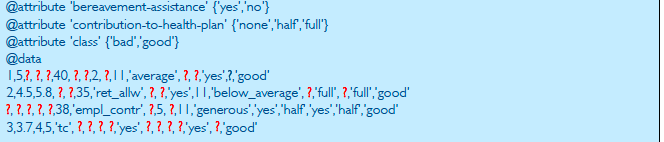
\includegraphics[width=.5\linewidth]{arffmissing}
%\end{figure}
In classification data have been labeled according to a certain \textbf{concept} ( good vs bad, positive vs negative etc...) identified by a \textbf{supervisor} who labeled the data.\\
The goal of classification is to compute a model using known that can \textbf{discriminate} between examples that have been labeled differently
\begin{figure}[H]
  \centering
 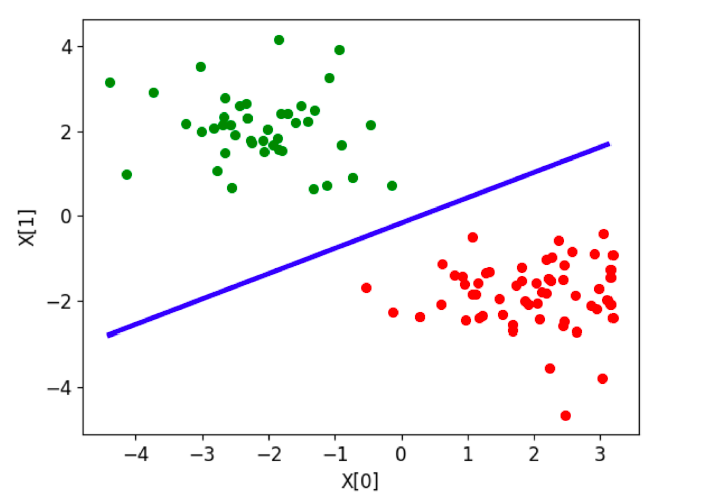
\includegraphics[width=.5\linewidth]{class1}
\end{figure}
The model is then used to \textbf{label unseen point} in the prediction phase.Differently form regression where the target variable is \textbf{continuous} , in classification the target variable is \textbf{discrete}.\\
An example using \textbf{classification rules}:
\begin{figure}[H]
  \centering
 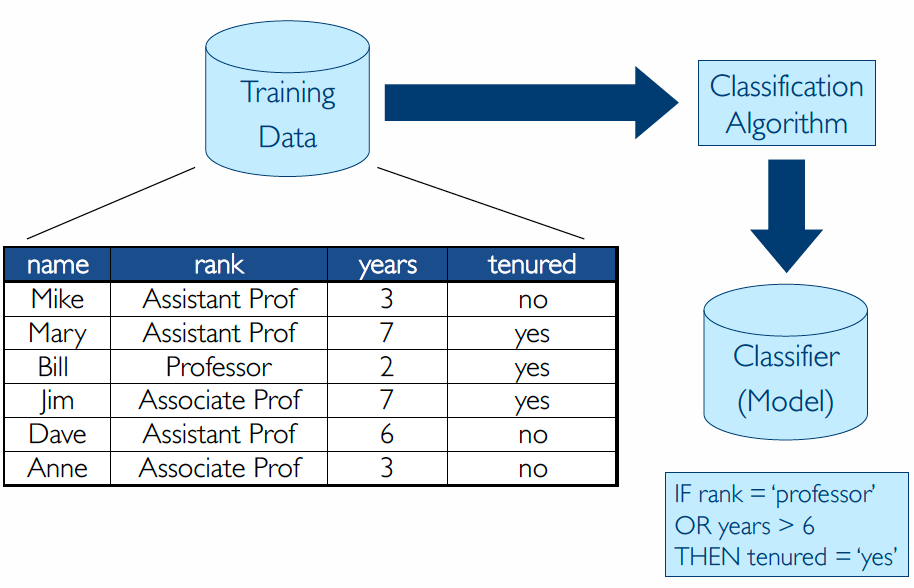
\includegraphics[width=.6\linewidth]{class2}
\end{figure}

\subsection{Model evaluation}
\begin{itemize}
\item \textbf{Accuracy}
\item \textbf{Speed} (of fitting and prediction)
\item \textbf{Robustness,scalability... }
\end{itemize}

\subsection{Logistic Regression}
The most simple classification algorithm. Starting from the basic idea behind classification algorithms :
\begin{figure}[H]
  \centering
 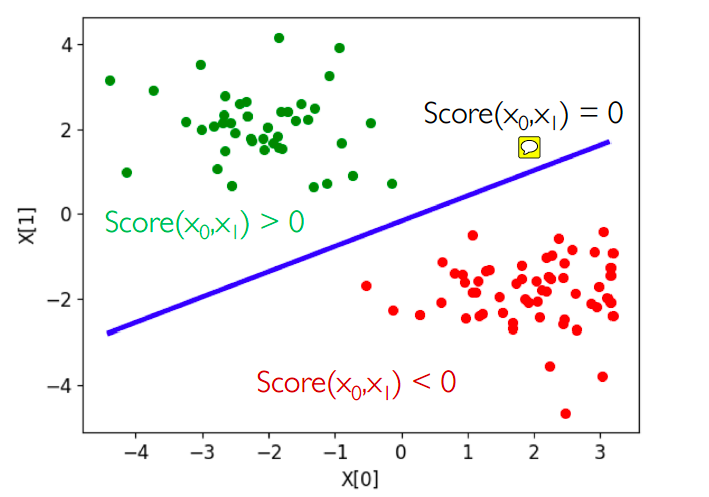
\includegraphics[width=.6\linewidth]{class3}
\end{figure}
$$ Score(\overrightarrow{x_i})= \sum \limits_{j=0}^{D}w_jh_j(\overrightarrow{x_i})$$
The label is determined as follows:

\[ \hat{y} = \text{sign}(Score(\overrightarrow{x_i})) =
  \begin{cases}
    +1       & \quad \text{if } Score(\overrightarrow{x_i}) \geq 0 \\
    -1  & \quad \text{if } Score(\overrightarrow{x_i}) < 0
  \end{cases}
\]
Logistic regression behaves similarly but instead of computing a label the algorithm computes the \textbf{probability of assigning a class to an example}:
$$ P(y_i | \overrightarrow{x_i})$$
For example for the positive class $+1$ : 
$$ P(\hat{y}_i = +1|\overrightarrow{x_i})= \frac{1}{1+e^{-Score(\overrightarrow{x_i})}}$$
Now adding explicitly feature transformations and weights:
$$ P(\hat{y}_i = +1|\overrightarrow{x_i},\overrightarrow{w})= \frac{1}{1+e^{-\overrightarrow{w}h(\overrightarrow{x_i})}}$$
The weights are computed using \textbf{maximum likelihood} :
$$ l(\overrightarrow{w}) = \prod \limits_{i=0}^{N} P(y_i|\overrightarrow{x_i},\overrightarrow{w})$$
This is maximized using \textbf{gradient descent} using the log-likelihood:
$$ ll(\overrightarrow{w}) = ln (\overrightarrow{w})$$
which updates weights j using :
$$ \frac{\partial{ll(\overrightarrow{w})}}{\partial{w_j}}= \sum \limits_{I=1}^{N}h_j(\overrightarrow{x_i})\left( 1[y_i=+1]-P(y=+1|\overrightarrow{x_i},\overrightarrow{w})\right)$$
So 
\[ \hat{y} =
  \begin{cases}
    +1       & \quad \sum \limits_{j=0}^{D}w_jh_j(x) \geq 0 \\
    -1  & \quad \sum \limits_{j=0}^{D}w_jh_j(x) < 0 
  \end{cases}
\]

\subsection{Overfitting and regularization}
Like regression :
\begin{itemize}
\item \textbf{L1 Regularization } : $l(\overrightarrow{w}) - \alpha||\overrightarrow{w}||_1$
\item \textbf{L2 Regularization} : $l(\overrightarrow{w})- \alpha||\overrightarrow{w}||^2_2$
\end{itemize}

\subsection{Multiclass Classification}
Logistic regression assumes that the output classes are just \textbf{two}. If there are more than 2 target classes, multiclass classification must be used.
A possibility is to use the \textbf{One vs the rest } method :
\begin{itemize}
\item For each class it creates \textbf{one classifier} that predicts the target class against all others
\item Then given an example \textbf{all classifiers} are used and the label with the \textbf{highest probability} is returned
\end{itemize}
In alternative a \textbf{multinomial multiclass} model can be used.

\subsection{Categorical values}
If the variables are \textbf{categorical} instead of numerical a good solution is to use \textbf{One Hot Encoding} which maps categorical values into \textbf{binary 0/1} values , each one describing a specific attribute. 
For example the feature \texttt{Outlook} can hold three values $\{$ Sunny,Rainy,Overcast$\}$  : 
\begin{itemize}
\item Outlook-sunny $\in \{ 0,1\}$
\item Outlook-rainy $\in \{ 0,1\}$
\item Outlook-overcast $\in \{ 0,1\}$
\end{itemize}


